\chapter{Related Work}
\label{related_work}
Motion planning is a widely researched topic with roots in control, artificial intelligence, computational geometry and Robotics. The literature presented in \cite{book_robot_motion_planning}, \cite{book_lavelle_planning} review significant portion of standard planning techniques. Due to the complexity of the autonomous cars and the environments, general techniques from robotics cannot be applied. Planning for autonomous cars in general is sub divided into two categories namely planning in unstructured environments such as parking areas etc and structured environments such as Road Networks where the traffic rules have to be followed. This chapter mainly focuses on the planning techniques in structured urban environments. 

\section{Planning Approaches}
\label{planning_aproaches}

Autonomous vehicles have been in research communities from 80's with projects such as PROMETHEUS \cite{prometheus}, the research was accelerated by the DARPA Grand Challenge in 2006 and DARPA Urban Challenge(DUC) in 2007 \cite{darpa_urban_challenge}. In DUC, six autonomous vehicles from different universities have completed the challenge and have used various techniques to accomplish the task. These techniques have formed the basis for modern day autonomous cars which perform much sophisticated compared to the DUC participants. 

Approach followed by different participants of DUC are described in \cite{darpa_urban_challenge}. Planning module of Boss, autonomous vehicle from Carnegie Melon University which won the DUC is described in general here. Its planning framework is mainly subdivided into 3 sub modules 

\begin{itemize}
	\item Mission control is the higher level module which creates a global path, assigns lane to the vehicle to reach the check points, detects blockades.
	\item Behavioral module is responsible for decisions such as precedence at intersections, lane change decision, speed planning, look ahead point assignment etc. 
	\item Motion planning module is responsible for generating local trajectories and converting them to steering and acceleration values. It initially creates a forward looking path and velocity planning is performed on top of that. 
\end{itemize}

After DUC, the research efforts have been increased to develop state of the art solutions in perception, planning and control for autonomous vehicles. Motion planning plays a crucial role in the system with aim of developing trajectories that are collision free and also fall under kinematic and dynamic constraints of vehicle, road boundaries and traffic rules \cite{motion_planning_techniques}. There has been a huge amount of research published with various techniques to solve the planning problem of autonomous vehicles. Potential fields is one of such algorithm, it models whole map as function of potential field with attractive forces towards goal and repulsive towards obstacles \cite{potential_field_3} \cite{potential_field_1} \cite{potential_field_2}. Path is found by traveling along the steepest gradient of potential field, however there is risk of paths getting trapped in local minima. Grid based approach is another generally used approach in Robotics, where the environment is perceived as set of grids and path is found traveling across these grids using algorithms like A*. The down side of these approach is that the complexity increases exponentially with increase in grid resolution and grid size, there have been different variants of this approach solving  problems with grid based approaches as discussed in \cite{A_star} \cite{D_star_1} \cite{kolski_thesis}. A comprehensive study of various approaches in motion planning for autonomous vehicles is presented in \cite{motion_planning_techniques} \cite{survey_planning_techniques}. 

 Planning approaches that are widely used in autonomous driving are classified as shown in Figure \ref{related_work_classification}. The following sub sections discuss research in each of the described sub-categories. 

\begin{figure}[H]
	\centering
	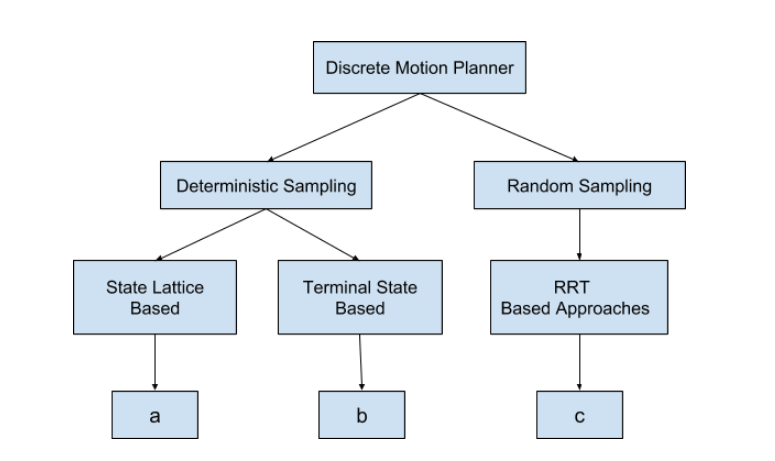
\includegraphics[width=0.8\textwidth]{Images/related_work/planning_division.png}
	\caption{General Overview of On-road planners. a - \cite{cmu_parallel_thesis}  \cite{diss_shui_phd_thesis} \cite{traj_planner_optimization} \cite{lattice_Gu_Tiyanu} \cite{unit_A_star} , b - \cite{kolski_thesis} \cite{real_time_traj_plan_article} \cite{darpa_urban_challenge}, c -\cite{rrt_star} \cite{rrt_urban_driv} \cite{mit_rrt}
	}
	\label{related_work_classification}
\end{figure}

\subsection{Random Sampling Approaches}
\label{rw_incremental_search}
Rapidly exploring random Tree(RRT) technique was initially introduced by Steven M. LaValle in his work presented in \cite{Lavalle_rrt}. RRT builds a tree incrementally by sampling new states. In each iteration a new sample $x$ is sampled and connected to the nearest neighbor $x_\textsubscript{neartest}$ in tree if it is collision free. The tree starts at the start location and is built till the path to goal location is found. Probablistic Roadmaps algorithm\cite{prm}(PRM) is another approach where uniform sampling is performed across the state space and are connected if a collision free path exists. Then a graph search algorithm is employed to find path from source to destination. Both of these approaches are probabilistic complete, i.e., as the number of samples increases probability of finding a solution approaches 1 given problem is solvable. 

Different variants of RRT's are widely accepted in robot motion planning because of its ability to explore higher dimensional problems at ease\cite{rrt_higher_dimension}. To improve the performance of RRT, bidirectional of two trees(Bi-RRT) has been proposed, though it improves the performance, handling discontinuities of two trees proved to be difficult\cite{birrt}. Environmentally guided RRT(EG-RRT) has been applied in real world scenarios\cite{egrrt}. MIT has applied a closed loop prediction model into RRT(CL-RRT) in its autonomous vehicle at DUC \cite{mit_rrt}, a snippet of planning is shown in Figure \ref{mit_rrt_fig}. Here motion models are used to generate trajectories and are evaluated for feasibility and performance. A variant named RRT* \cite{rrt_star} has been proposed which guarantee asymptotic optimality.  In this approach each state stores cost from start and when a new sample is added, surrounding neighbors are tested if a better path can be found and tree is rewired. There have been many techniques to reduce the number of sampled states in-order to save computational time. Informed-RRT \cite{informed_rrt} reduces sampled space accordingly to the actual best path, states that are far away from the goal are not sampled.

\begin{figure}
	\centering
	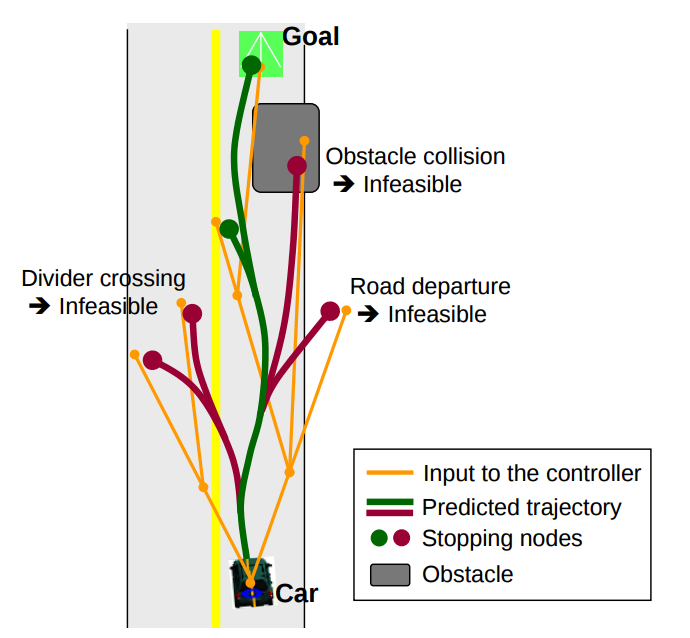
\includegraphics[width=0.6\textwidth]{Images/related_work/mit_urban_planning.png}
	\caption{MIT Darpa Urban Challenge - RRT based planning approach}
	\label{mit_rrt_fig}
\end{figure} 

In real world situations, environment is not completely predictable and the computed path need to be dynamically re-planned over the time. This needs either a new plan to be generated quickly or rapid correction of old path. The approach Anytime-RRT \cite{anytimerrt} creates an initial path using RRT and optimizes it on the go to create an optimal path, re-planning is triggered when path is no longer valid. The method RRT$^x$ \cite{rrtx} updates the search space when ever obstacle changes are observed and repairs the surrounding tree. 

Though RRTs are best performing algorithms in planning, they exhibit certain deficiencies in terms of motion planning for autonomous vehicles especially in on road driving conditions.  RRT-based planners generate jerky and unnatural trajectories that contain many unnecessary turns\cite{improved_rrt}, these are suitable for open areas such as parking areas. Road parallel trajectories are preferred in structured environments. 

\subsection{Lattice Planners}
\label{rw_lattice_planners}
The algorithm uses a discrete representation of the planning area with multiple states, often a multi dimensional one with dimensions such as position, acceleration, velocity, time etc. These states are connected together and the problem then reduces to finding a path from the initial state to the final state in the lattice. This approach is generally well suited for non-holonomic robots and highly constrained areas such as road networks\cite{lattice_1}. Lattice planners are resolution complete, i.e., they can be automatically adjusted to change in resolution to explore state space consistently. The approached proposed in \cite{lattice_1} uses a multi resolution state lattice with high resolution in start and goal ans lower resolution in middle. This reduces the computational complexity of planner. Continuity of path and curvature are constraints in path planning, these are addressed in the research \cite{lattice_2} by defining a 2-D input set U(heading and steering) over 4D configuration including 2D position, heading and steering. In \cite{cmu_parallel_thesis} the author added curvature to each state along with 2D position heading and curvature. Paths between the vehicle and sampled sates are connected using third order spirals. A range of times and velocities are assigned to each vertex to enable spatio temporal search. Constant acceleration profiles are chosen making it difficult for the vehicle to follow. Thus due to multitude of states involved the number of trajectories created are in order of few hundred thousands and increase exponentially if resolution is increased or new dimension is added. A graphical processing unit(GPU) is employed to run the evaluations in parallel to provide real-time response. 

To improve the performance of \cite{cmu_parallel_thesis}, the research published in \cite{traj_planner_optimization} utilizes quartic polynomials to ensure continuous curvature, connections are made from sampled end points and current state, Figure \ref{trajopt} shows further information about path and velocity representation. In this approach speed profiles are generated inversely and checks are included to ensure comfort, efficiency. The approach proposed in \cite{traj_smoothing} is a two level planning approach which generates optimal collison free reference path initially and then performs search across this reference path to find an optimal path. The reference path leads to focused search and more human like driving style. The research published in \cite{diss_shui_phd_thesis} further improves the trajectory smoothness ensuring high level of trajectory diversity. 

In summary lattice planners create trajectories that are smooth, optimal and complying to dynamic and kinematic abilities of vehicle. These approaches are well suited for structured and dynamic environments. These approaches are expensive and complexity increases exponentially with addition of new state or resolution. 

\begin{figure}
	\centering
	\begin{subfigure}{.5\textwidth}
		\centering
		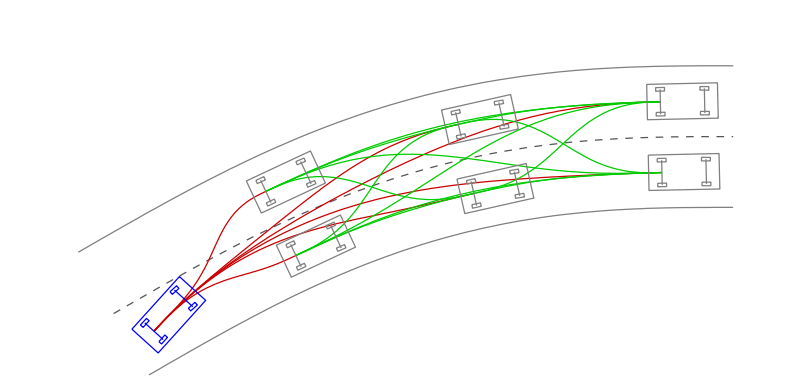
\includegraphics[width=1.0\linewidth]{Images/related_work/traj_optim_1.png}
		\caption{Path set. blue vehicle represents the current
			vehicle pose, and grey vehicles represent sampled endpoints.
			The red paths are quartic curvature polynomials and the
			green paths are cubic ones}
		\label{trajoptsub1}
	\end{subfigure}%
	\begin{subfigure}{.5\textwidth}
		\centering
		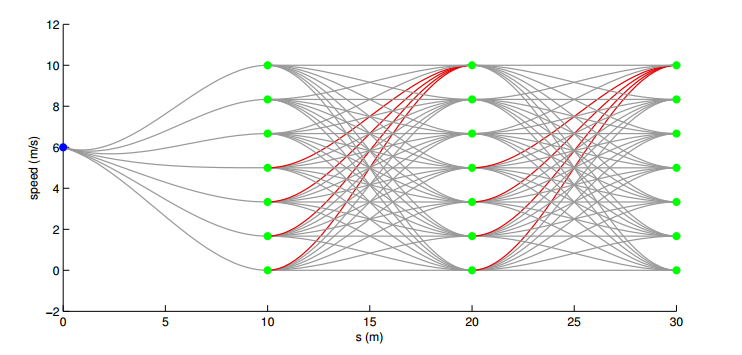
\includegraphics[width=1.0\linewidth]{Images/related_work/traj_optim_2.png}
		\caption{Speed set. The green points are sampled speeds, the
red curves are beyond the acceleration limit, and the grey
curves are valid ones}
		\label{trajoptsub2}
	\end{subfigure}
	\caption{Path velocity representation in \cite{traj_planner_optimization}}
	\label{trajopt}
\end{figure}

\subsection{Local Search}
\label{rw_local_search}

Local Search or forward projecting trajectories
Different types of curves, 
forward samples, 

Velocity planning - different approaches - check if needed

sampling
Action space - something similar to this thesis, 
State Space - final states

Combining Path and Velocity Werling, Lattices, Unit A* approach


%\subsection{Sampling Approaches}
%\label{sampling}



%\subsection{Trajectory Representation}
%\label{trajectory_rep}
%splines? polynomials? lattice?



\section{Trajectory Evaluation}
\label{traj_eval}

collison checking - different approaches 

cost functions - for different parameters


%Look if the sampling based, RRT based, lattice based etc etc should be combined together?
%write about MDP, POMDP etc 